\documentclass[big]{beamer}

\mode<presentation>{
  \usetheme{default}
  \usefonttheme{serif}
  \setbeamercovered{transparent}
%--------------------------------------------------
%   \setbeamerfont{institute}{size=\footnotesize}
%-------------------------------------------------- 
  \setbeamerfont{tableofcontents}{size=\Large}
}

\usepackage[english]{babel}
\usepackage{times}
\usepackage{algorithmic}
\usepackage{algorithm}
\usepackage{epsfig}
\usepackage{pgf}

% Latin-1 only
\usepackage[latin1]{inputenc}
\usepackage[T1]{fontenc}
%--------------------------------------------------
% % Chinese-support
% \usepackage[nocjkbg5]{ucs}
% \usepackage[utf8x]{inputenc}
% \usepackage[C00,T1]{fontenc}
% \newcommand\tradtext[1]{\bgroup\fontencoding{C00}\fontfamily{ming}\selectfont%
% \SetUnicodeOption{cjkbg5}#1\egroup}
%-------------------------------------------------- 

\title[]{Survey: The Markov Random Field Model for Term Dependencies}
\author[]{Ruey-Cheng Chen} 
\institute{Academia Sinica, Taiwan}
\date[]{}
\subject{Theoretical Computer Science}
%--------------------------------------------------
% \AtBeginSubsection[]
% {
%   \begin{frame}<beamer>
%     \frametitle{Outline}
%     \tableofcontents[currentsection,currentsubsection]
%   \end{frame}
% }
%-------------------------------------------------- 
%\beamerdefaultoverlayspecification{<+->}
\newcommand<>\ul[2]{\textbf{#1}\begin{itemize}#2\end{itemize} \vskip 0.5em}
\newcommand<>\ull[1]{\begin{itemize}#1\end{itemize}}
\newcommand<>\ol[2]{\textbf{#1}\begin{enumerate}#2\end{enumerate}}
\newcommand<>\oll[1]{\begin{enumerate}#1\end{enumerate}}
\newcommand<>\dl[2]{\textbf{#1}\begin{description}#2\end{description}}
\newcommand<>\f[2]{\begin{frame}{#1}#2\end{frame}}
\newcommand<>\mydef[2][]{\textbf{#1}\par#2\par}
%--------------------------------------------------
% \newcommand<>\mydef[2][]{\begin{definition}[#1]#2\end{definition}}
%-------------------------------------------------- 
\newcommand<>\tbl[3]{\textbf{#1}\vskip 0.5em\begin{center}\begin{tabular}{#2}#3\end{tabular}\end{center}}
\newcommand<>\fig[3]{\textbf{#1}\vskip 0.5em\begin{center}\begin{figure}\includegraphics[#2]{#3}\end{figure}\end{center}}
\newcommand<>\cols[1]{\begin{columns}#1\end{columns}}
\newcommand<>\col[2]{\begin{column}{#1}#2\end{column}}

\begin{document}

\frame{ \titlepage }

\f{References}{

  \ul{Mandatory Reference}{ 

    \item Metzler, D. and Croft, W. B. 2005. A Markov random field model for
    term dependencies. In \emph{Proceedings of SIGIR '05}.  ACM, New York, NY,
    472-479.  \item Metzler, D. and Croft, W. B. 2007. Latent concept expansion
    using markov random fields. In \emph{Proceedings of SIGIR '07}.  ACM, New
    York, NY, 311-318.
  
  }

  \ul{Pointers}{ 
    \item \footnotesize{\url{ http://ciir.cs.umass.edu/~metzler/ }}
    \item \footnotesize{\url{ http://ciir.cs.umass.edu/personnel/croft.html }}
  }
}

\f{Outline}{ \tableofcontents }

\section{Introduction}
\f{Introduction}{
  \ul{Motivation}{\item Modeling Term Dependence \item Many previous attempts \ldots}
  \ul{Proposed Method}{
    \item Modeling: The joint distribution $P_\Lambda(Q,D)$
    \item Training: Pairs of relevant documents and queries 
    \item Ranking: $P_\Lambda(D|Q)$
  }
}

\section{Background}
\subsection{Graph-Theoretical Concepts}
\f{Graph}{
  \ul{Basic Concepts}{
    \item An undirected graph $G = (V, E)$ is a collection of nodes $V$ and edges $E$.
    \item Two nodes $i, j \in V$ are \emph{neighbors} if $(i, j) \in E$.
    \item Neighborhood of a node $i$: $\{j \mid (i, j) \in E\}$.
    \item A node is not a neighbor of itself, i.e., $(i, i) \notin E$.
    \item A clique of $G$ is either a single node or a complete subgraph of $G$.
  }
  \begin{figure}
    \centering
    \includegraphics[width=100pt]{clique}
  \end{figure}
}

\subsection{Random Fields}
\f{Random Fields}{
  \mydef[Random Fields]{
    Let $F = \{X_1, \ldots, X_m\}$ be a set of random variables defined on the
    sample space $\Omega$, in which each $X_i$ takes a value $x_i \in
    \mathcal{L}$.  A probability measure $p$ is a \emph{random field} if
    $p(\omega) > 0$ for all $\omega \in \Omega$.
  }
  \vskip1em
  \ul{Random Fields on $G$}{
    \item Assign each random variable $X_i$ to a node of $G$.
    \item Values of random variables are usually spatially correlated.
  }
  \begin{figure}
    \centering
    \includegraphics[width=100pt]{rf}
  \end{figure}
}

\f{Markovianity}{
  \ul{Neighborhood System}{
    \item $\mathcal{N}_i = \{j \mid (i, j) \in E\}$.
    \item Symmetric relation: $i \in \mathcal{N}_j \Leftrightarrow j \in \mathcal{N}_i$
  }
  \ul{Pairwise Markovianity}{
    \item $(i, j) \notin E \Rightarrow$ ``$X_i$ and $X_j$ are independent, when conditioned on all others'', i.e., 
    $p(X_i, X_j \mid X_{F - \{i, j\}}) = p(X_i \mid X_{F - \{i, j\}}) p(X_j \mid X_{F - \{i, j\}})$.
  }
  \ul{Local Markovianity}{
    \item ``Given the neighborhood of $i$, $X_i$ is independent of the rest``,
    i.e., $p(X_i, X_{F - \{i\} \cup \mathcal{N}(i)} \mid X_{\mathcal{N}(i)}) =
    p(X_i \mid X_{\mathcal{N}(i)}) p(X_{F - \{i\} \cup \mathcal{N}(i)} \mid
    X_{\mathcal{N}(i)})$.
    \item Equivalent form: $p(X_i \mid X_{F - \{i\}}) = p(X_i \mid X_{\mathcal{N}(X_i)})$.
  }
}

\subsection{Markov Random Fields}
\f{Markov Random Fields}{
  \mydef[Markov Random Fields]{
    A random field $F$ is said to be \emph{Markov} on $\Omega$ with respect to
    a neighborhood system $\mathcal{N}$ if and only if $p(\mathbf{x}) > 0$ for
    all $\mathbf{x}$ and $F$ has the local Markov property.
  }
  \vskip1em
  \mydef[Hammersley-Clifford Theorem]{
    Given a random field $F$ defined on $\Omega$.
    \oll{
      \item If $F$ is a Markov random field, $p(\mathbf{x})$ can be written as
      a Gibbs distribution \[p(\mathbf{x}) = \frac{1}{Z} \prod\limits_{c \in
      \mathcal{C}} e^{ -\psi_c(\mathbf{x}_c)},\] where $Z$ is a
      \emph{normalizing constant} called \emph{partition function}, functions
      $\psi_c(\dot)$ are \emph{clique potential}, and $\mathcal{C}$ is the set
      of all cliques of $G$.  The negative of the exponents are called \emph{energy}.
      \item If $p(\mathbf{x})$ can be written in Gibbs form for the cliques of some graph, it has the global Markov property.
    }
  }
}

\f{Hammersley-Clifford Theorem}{
  \ul{Impact}{
    \item A Markov random field can be specified via the clique potentials.
  }
  \ul{More derivation}{
    \item The local Markovian conditionals can be computed as \[p(X_i \mid
    X_{\mathcal{N}(i)}) = \frac{1}{Z_{X_{\mathcal{N}(i)}}} \prod\limits_{c; i \in
    c} e^{-\psi_c(\mathbf{x}_c)}.\]
    \item Note that the normalizing constant depends on $X_{\mathcal{N}(i)}$.
  }
}

\section{Proposed Method}
\subsection{MRF Model in IR}
\f{MRF in IR}{
  \mydef[The Joint $P_\Lambda(D,Q)$]{
    \begin{equation*} P_\Lambda(Q,D) = \frac{1}{Z_\Lambda} \prod\limits_{c \in C(G)} \psi(c;\Lambda) \end{equation*}
    where $Q = q_1 \ldots q_n$, $C(G)$ is the set of cliques in $G$, each
    $\psi(\cdot;\Lambda)$ is a non-negative \emph{potential function} over
    clique configuration parameterized by $\Lambda$, and $Z_\Lambda =
    \sum_{Q,D} \prod_{c \in C(G)} \psi(c;\Lambda)$ is the \emph{normalizing
    factor}.
  }
  \vskip1em
  \ul{Explanation}{
    \item In a clique, every node depends on (links to) the others.
    \item 1-clique is not of interest in the context.
    \item The Gibbs form are usually expressed as log-linear models, i.e., \[\prod_c e^{\psi(c)} \equiv e^{\sum_c \psi(c)}.\]
  }
}

\subsection{Ranking}
\f{Ranking}{
  \mydef[Ranking by using the Posterior]{
    \begin{eqnarray*}
      P_\Lambda(D \mid Q) &=& \frac{P_\Lambda(Q,D)}{P_\Lambda(Q)} \\
      &\approx& \log P_\Lambda(Q,D) - \log P_\Lambda(Q) \\
      &\approx& \sum\limits_{c \in C(G)} \log \psi(c;\Lambda) \\
    \end{eqnarray*}
  }
  \vskip1em
  \ul{Explanation}{
    \item The logarithmic function is monotonic (at line 2).
    \item $\log P_\Lambda(Q)$ does not depend on $D$.
    \item The normalizing factor is a constant.
  }
}

\f{Ranking (cont'd)}{
  \mydef[Potential Function and Feature Function]{
    Potential functions are most commonly parameterized as \[\psi(c; \Lambda) =
    \exp[\lambda_c f(c)],\] where $f(c)$ is some real-valued \emph{feature
    function} over clique value, and $\lambda_c$ is the weight given to that
    particular feature.  Therefore, the ranking formula becomes:
    \[ P_\Lambda(D \mid Q) = \sum\limits_{c \in C(G)} \lambda_c f(c). \]
  }
  \ul{Using the MRF Model}{
    \item Construct a graph that represents the term dependencies.
    \item Define a set of potential functions.
    \item Rank documents according to the posterior.
  }
}

\subsection{Dependences and Potentials}
\f{Graph Structure}{
  \ol{Dependence Assumptions}{
    \item Full independence (FI)
    \item Sequential dependence (SD)
    \item Full dependence (FD)
  }
  \begin{figure}
    \centering
    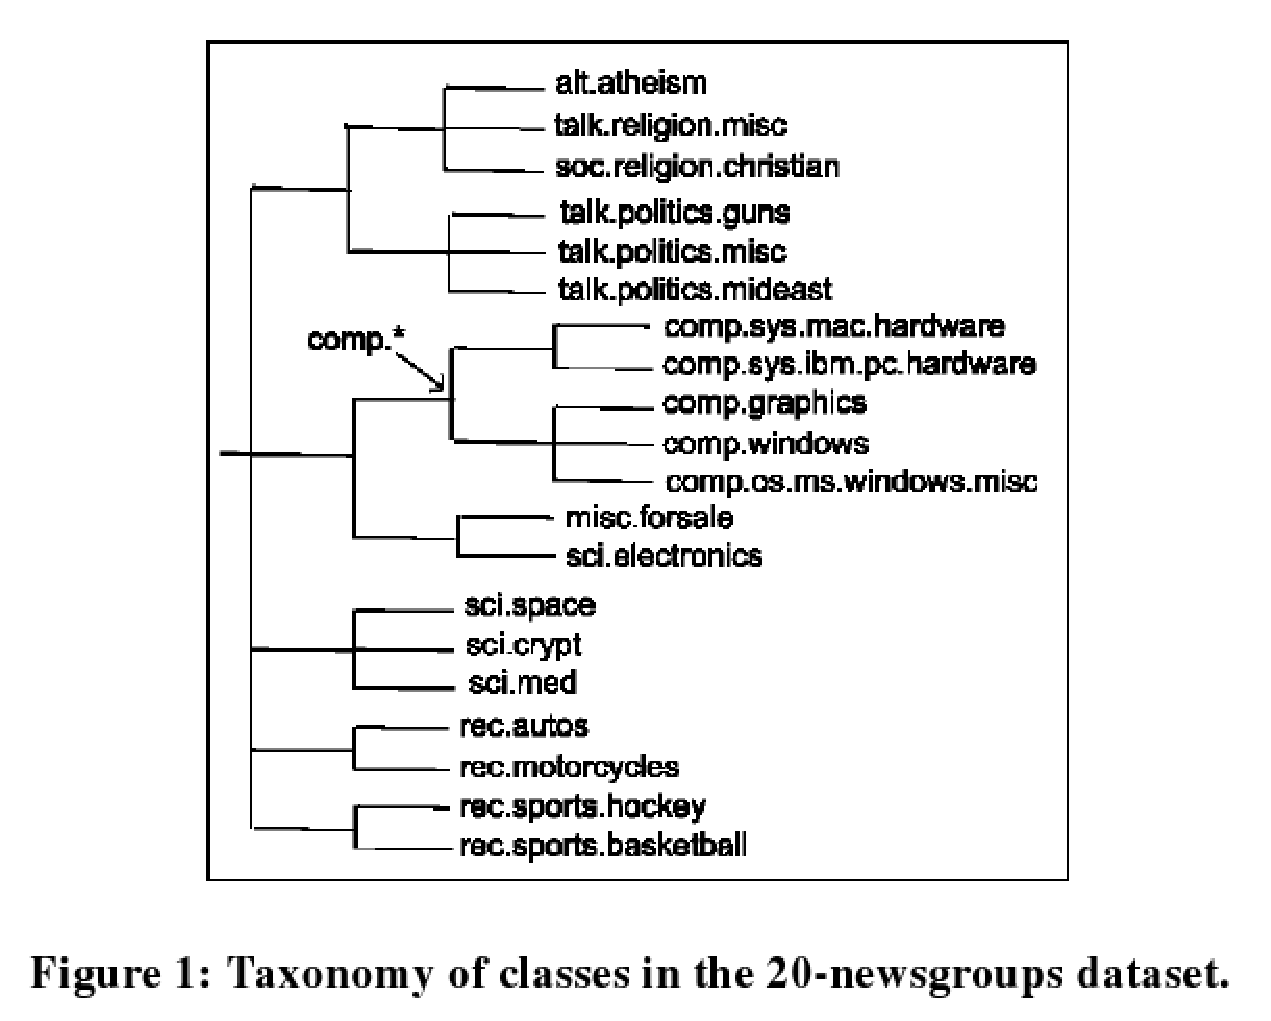
\includegraphics[width=300pt]{fig1}
  \end{figure}
}

\f{Potential Functions}{
  \ul{Compatibility}{
    \item A good potential function assigns high values to the most \emph{compatible} clique, e.g.,
    \[\psi(\text{information}, \text{retrieval}, D) > \psi(\text{information}, \text{assurance}, D).\]
    \item Potential functions can be computed efficiently.
    \item In this work, ``compatibility'' means ``term co-occurrence''.
  }
  \ul{Proposed Potentials}{
    \item FI: $\psi_T(c) = \lambda_T \log P(q_i \mid D)$.
    \item SD: $\psi_O(c) = \lambda_O \log P(\#1(q_i, \ldots, q_{i+k}) \mid D)$.
    \item FD: $\psi_U(c) = \lambda_U \log P(\#uwN(q_i, \ldots, q_j) \mid D)$.
  }
}

\f{Potential Functions (cont'd)}{
  \mydef[Detailed Derivation]{
    \begin{eqnarray*}
    \psi_T(c) &=& \lambda_T \log P(q_i \mid D) \\
    &=&  \lambda_T \log [(1-\alpha_D) \frac{tf_{q_i,D}}{|D|} + \alpha_D \frac{cf_{q_i}}{|C|} ] \\
    \psi_O(c) &=& \lambda_O \log P(\#1(q_i, \ldots, q_{i+k}) \mid D) \\
    &=&  \lambda_O \log [(1-\alpha_D) \frac{tf_{\#1(q_i \ldots q_{i+k}), D}}{|D|} + \alpha_D \frac{cf_{\#1(q_i \ldots q_{i+k})}}{|C|} ] \\
    \psi_U(c) &=& \lambda_U \log P(\#uwN(q_i, \ldots, q_j) \mid D) \\
    &=&  \lambda_O \log [(1-\alpha_D) \frac{tf_{\#uwN(q_i \ldots q_j), D}}{|D|} + \alpha_D \frac{cf_{\#uwN(q_i \ldots q_j)}}{|C|} ] \\
    P_\Lambda(D \mid Q) &=& \sum_c \lambda_c f(c) \\
    &=& \sum_{c \in T} \lambda_T f_T(c) + \sum{c \in O} \lambda_O f_O(c) + \sum{c \in O \cup U} \lambda_U f_U(c) \\
    \end{eqnarray*}
  }
}

\section{Evaluation}
%--------------------------------------------------
% \f{Setup}{ \fig{}{width=300pt}{tbl2} }
%-------------------------------------------------- 
\f{Evaluation: Results}{ \fig{}{width=300pt}{tbl3} }
\f{Evaluation: Results (cont'd)}{ \fig{}{width=300pt}{tbl4} }
\f{Evaluation: Results (cont'd)}{ \fig{}{width=300pt}{tbl5} }
\f{Evaluation: Results (cont'd)}{ \fig{}{width=300pt}{tbl6} }

\section{Conclusion}

%--------------------------------------------------
% \f{Problem Definition (cont'd)}{
%   \ul{Similar Problems}{
%     \item \emph{k-budgeted cover}: cover as many nodes in $Y_t$ using $k$ nodes from $X_t$
% 
%     \item \emph{$\rho$-partial cover}: cover at least $\rho|Y_t|$ nodes in
%     $Y_t$ using as few nodes from $X_t$ as possible, given any $\rho \le 1$
% 
%     \item Both problems are NP-Hard
%   }
%   \ul{Notations}{
%     \item $N(x)$: the set of new nodes efficiently discoverable from $x$
%     \ull{ \item i.e., $N(x)= \{y \mid (x,y) \in Z_t \}$ }
%     \item $N(S) = \cup_{x \in S}N(x)$ for a subset $S$ of $X_t$
%   }
%   \mydef[Key Metric: Overhead]{
%     If a set $O$ of old pages are crawled to discover $|N(O)|$ pages, we define the \emph{overhead} of $O$ as $\frac{|O|}{|N(O)|}$.
%   }
% }
% 
% \subsection{\texttt{GREEDY} Algorithm}
% \f{An Algorithmic Upper Bound}{
%   \textbf{The \texttt{GREEDY} Algorithm}
%   \vskip 0.5em
%   \begin{algorithmic}[1]
%     \STATE $C_t \leftarrow \emptyset$
%     \WHILE{``not done''}
%       \STATE Find $x \in X_t \backslash C_t$ that maximize $|N(X) \backslash N(C_t)|$
%       \STATE $C_t \leftarrow C_t \cup \{x\}$
%     \ENDWHILE
%     \STATE \textbf{return} $C_t$
%   \end{algorithmic}
%   \vskip 1em
% 
%   \ul{Predicate ``not done''}{
%     \item $|C_t| < k$ in $k$-budgeted cover problem
%     \item $|N(C_t)| < \rho|Y_t|$ in $\rho$-partial cover problem
%   }
% }
% 
% \section{Data}
% \f{Data}{
%   \ul{Site Recrawl Dataset}{
%     \item A repeated recrawl of 200 websites over a period of manyweeks
%     \item Noise site and ``Orphan'' pages removed
%     \item 42 out of 77 sites selected after data cleaning
%     \item 640,389 pages at the first timestamp, and 223,435 new pages over the period
%   }
%   \ul{Chilean Web Dataset}{
%     \item 3 snapshots for the Chilean Web based on monthly complete crawls
%     \item 7.4M pages and 67.5M edges in the first snapshot
%     \item 7.43M pages and 70.66M edges in the first snapshot
%   }
% }
% 
% \section{Measurements}
% \subsection{Cover Size}
% \f{Measurements: Cover Size}{
%   \fig{Cover Size vs. the Number of Pages Covered}{width=250pt}{fig/fig2-1.eps}
% }
% 
% \f{Measurements: Cover Size (cont'd)}{
%   \fig{Cover Size vs. the Number of Pages Covered}{width=250pt}{fig/fig2-2.eps}
% }
% 
% \f{Measurements: Cover Size (cont'd)}{
%   \fig{Overhead and the Number of Covered Pages}{width=250pt}{fig/fig3a.eps}
% }
% 
% \f{Measurements: Cover Size (cont'd)}{
%   \fig{Fraction of New Pages Covered}{width=250pt}{fig/fig3b.eps}
% }
% 
% \subsection{90\% Covers}
% \f{Measurements: 90\% Covers}{
%   \fig{90\% Covers Statistics}{width=250pt}{fig/fig3c.eps}
% }
% 
% \f{Measurements: 90\% Covers (cont'd)}{
%   \fig{Histogram of 90\% Cover Sizes}{width=250pt}{fig/fig4.eps}
% }
% 
% \subsection{Node Redundancy}
% \f{Measurements: Node Redundancy}{
%   \fig{Overlap Distribution}{width=250pt}{fig/fig5.eps}
% }
% 
% \subsection{Overhead}
% \f{Measurements: New Page Discovery}{
%   \fig{Global Discovery of New Pages on Old Sites}{width=250pt}{fig/fig6.eps}
% }
% 
% \f{Measurements: New Site Discovery}{
%   \fig{Chile Site-Level Discovery}{width=250pt}{fig/fig7.eps}
% }
% 
% \section{History-Based Algorithms}
% \f{History-Based Algorithms}{
%   \ul{Using Statistics in $H_{t-i}$ for Discovery of New Content in $H_t$}{
%     \item \texttt{OD}: the number of pages discovered historically
%     \item \texttt{CLIQ}: past degree information and overlaps of pages discovered
%     \item \texttt{COV}: historical results of \texttt{GREEDY}
%   }
%   \ul{Notations}{
%     \item $S^*$: the optimal solution to the $k$-budgeted cover on $H_t$
%     \item $S$: the solution returned by an algorithm \texttt{ALG}
%     \item $\rho(\mathtt{ALG}) = N(S)/N(S^*)$ (coverage)
%     \item $N$: the total number of new nodes
%   }
% }
% 
% \f{Algorithms}{
%   \mydef[\texttt{OD}: Outdegree-Based Algorithm]{
% 
%     Suppose that for every old node $i$, we have an estimate $p_i = |N(i)|/N$.
%     A natural algorithm is as follows: pick $k$ old nodes with the largest
%     $p_i$'s and crawl these nodes.
% 
%   }
%   \vskip1em
% 
%   \mydef[\texttt{CLIQ}: Overlap-Based Algorithm]{
% 
%     Let $p_i$ be as above, and for a pair of old nodes $(i,j)$, let $p_{ij}$ be
%     the fraction of new nodes that $i$ and $j$ both cover: $p_{ij} = |N(i) \cap
%     N(j)|/N$.  Partition nodes into equivalence classes $C_1, \ldots, C_l$, and
%     sort these classes in order of descending $N(i)$'s.  The output $S$ is the
%     set of $p_i$'s corresponding to the $k'$ largest $q_i$'s, where $k' =
%     \min(k,l)$ and $q_i = \max_{j \in C_i}p_j$.
% 
%   }
% 
% }
% 
% \section{Analysis}
% \f{Results}{
%   \fig{Coverage as a Function Of Average Cover Size, Recrawl Frequency 1}{width=250pt}{fig/fig8.eps}
% }
% 
% \f{Results (cont'd)}{
%   \fig{Coverage as a Function Of Average Cover Size, Recrawl Frequency 4}{width=250pt}{fig/fig9.eps}
% }
% 
% \f{Results (cont'd)}{
%   \fig{Analysis of Covers}{width=\columnwidth}{fig/tbl2.eps}
% }
%-------------------------------------------------- 

\section<presentation>*{\appendixname}

\begin{frame}%[allowframebreaks]
  \frametitle{References}
  \small
  \bibliography{report}
  \bibliographystyle{alpha}
\end{frame}

\frame{
  \begin{center}
    \Huge{Thanks for your attention!}
    \par
    Any Question?
  \end{center}
}

\end{document}
